\chapter{O fecho: a promessa com os buracos abertos}\label{cap:fecho}

Dezenove capítulos mediram buracos separados: a memória que cega, o atraso do dado, o pedaço
escolhido, a mudança que chega sem avisar, a cauda que vem junto, o passado que não volta, o trabalho
que se gasta. Cada um tem o seu preço medido, e nenhum foi medido junto com os outros.

Este capítulo mede a promessa do primeiro capítulo com \textbf{três buracos abertos ao mesmo tempo}: a
janela da calibração, o atraso do dado e o mundo. A promessa é a mesma em todas as
\numFechoConfiguracoes{} configurações --- \numPromessaPct{}\% dos dias rompendo o corte, que é
\numFechoPromessa{} em fração ---, com \numFechoJanelas{} tamanhos de
janela em mundos de \numFechoDias{} dias. O posto acompanha a janela, mas ele é um número inteiro:
arredondado para cima, o corte assina sozinho \numFechoAssinadoCurta{} na janela curta,
\numFechoAssinadoMedia{} na média e \numFechoAssinadoLonga{} na longa. A pergunta é se os buracos somam ou se compõem.

\section{A medição da pilha}

\begin{table}[htbp]
  \centering
  \small
  \begin{tabular}{lrrrr}
    \hline
    mundo & janela & atraso & entrega & em vezes \\
    & (dias) & (dias) & medida & a promessa \\
    \hline
    parado & \numFechoJanelaCurta{} & nenhum & \numFechoEntregaParadoCurtaSemAtraso & \numFechoParadoCurtaSemAtraso \\
    parado & \numFechoJanelaCurta{} & \numFechoAtraso{} & \numFechoEntregaParadoCurtaComAtraso & \numFechoParadoCurtaComAtraso \\
    parado & \numFechoJanelaMedia{} & nenhum & \numFechoEntregaParadoMediaSemAtraso & \numFechoParadoMediaSemAtraso \\
    parado & \numFechoJanelaMedia{} & \numFechoAtraso{} & \numFechoEntregaParadoMediaComAtraso & \numFechoParadoMediaComAtraso \\
    parado & \numFechoJanelaLonga{} & nenhum & \numFechoEntregaParadoLongaSemAtraso & \numFechoParadoLongaSemAtraso \\
    parado & \numFechoJanelaLonga{} & \numFechoAtraso{} & \numFechoEntregaParadoLongaComAtraso & \numFechoParadoLongaComAtraso \\
    mudado & \numFechoJanelaCurta{} & nenhum & \numFechoEntregaMudadoCurtaSemAtraso & \numFechoMudadoCurtaSemAtraso \\
    mudado & \numFechoJanelaCurta{} & \numFechoAtraso{} & \numFechoEntregaMudadoCurtaComAtraso & \numFechoMudadoCurtaComAtraso \\
    mudado & \numFechoJanelaMedia{} & nenhum & \numFechoEntregaMudadoMediaSemAtraso & \numFechoMudadoMediaSemAtraso \\
    mudado & \numFechoJanelaMedia{} & \numFechoAtraso{} & \numFechoEntregaMudadoMediaComAtraso & \numFechoMudadoMediaComAtraso \\
    mudado & \numFechoJanelaLonga{} & nenhum & \numFechoEntregaMudadoLongaSemAtraso & \numFechoMudadoLongaSemAtraso \\
    mudado & \numFechoJanelaLonga{} & \numFechoAtraso{} & \numFechoEntregaMudadoLongaComAtraso & \numFechoMudadoLongaComAtraso \\
    \hline
  \end{tabular}
  \caption{A promessa medida nas \numFechoConfiguracoes{} configurações, em
    \numFechoSementes{} mundos sorteados por célula, na janela de \numFechoHorizonte{} dias que segue
    a mudança. A última coluna é a entrega dividida pela promessa, e a dispersão entre os mundos,
    no mundo parado e sem atraso, é de \numFechoDispersaoParadoCurtaSemAtraso{} na janela curta e de
    \numFechoDispersaoParadoLongaSemAtraso{} na longa.}
  \label{tab:pilha}
\end{table}

A primeira metade da tabela traz o mundo parado, e ali a lição é conhecida: \textbf{o que se quer é
entregar a promessa}, e a mais perto dela é a melhor --- a janela longa entrega
\numFechoParadoLongaSemAtraso{} vezes a promessa e a curta \numFechoParadoCurtaSemAtraso{}. A diferença
entre as duas, medida nos mesmos \numFechoSementes{} mundos sorteados, é de \numFechoParadoDiferenca{}
vezes, ou \numFechoParadoDiferencaDesvios{} erros-padrão da média, com dispersão de
\numFechoParadoDiferencaDispersao{} entre os mundos: é o limite do que \numFechoSementes{} mundos
separam. O atraso não move nada de importante.

A segunda metade inverte a ordem. Com o mundo dobrando, a janela longa entrega
\numFechoMudadoLongaSemAtraso{} vezes a promessa e a curta \numFechoMudadoCurtaSemAtraso{}: \textbf{a
memória que era melhor no mundo parado é a pior no mundo que mudou}. O motivo é o mesmo de sempre
--- a janela longa carrega mais dias de antes da mudança, e é por isso que ela demora mais para
esquecer o mundo que já não existe.

\begin{figure}[htbp]
  \centering
  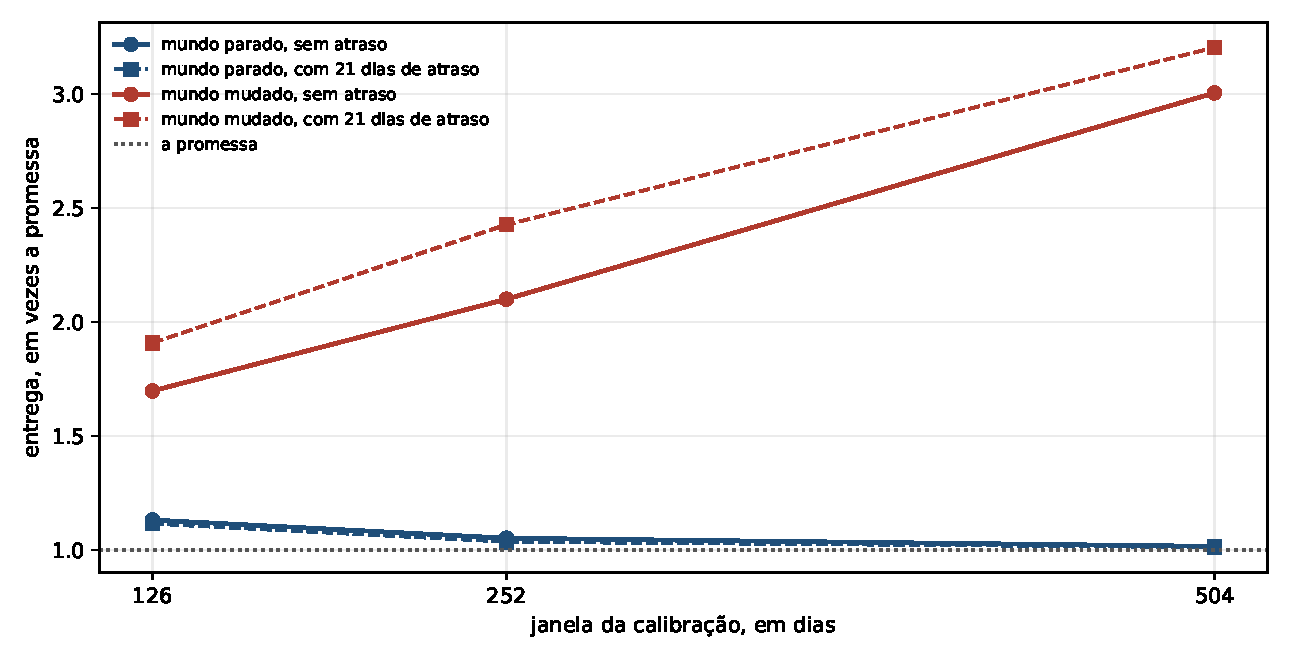
\includegraphics[width=\linewidth]{figuras/E20_o_fecho_1.pdf}
  \caption{A entrega contra a janela da calibração, nos dois mundos e com e sem atraso. As duas
    curvas do mundo parado descem e as duas do mundo que muda sobem: o mesmo eixo, o sentido
    trocado.}
  \label{fig:cruzamento}
\end{figure}

O cruzamento é a coisa toda do capítulo. Num mundo que não muda, aumentar a memória melhora a
entrega; num mundo que muda, aumentar a memória piora. E o sinal do efeito depende de uma coisa que
o instrumento só descobre depois: se o mundo vai mudar.

\section{Os buracos se compõem}

Falta a conta que o título promete. Cada buraco foi medido sozinho, no mundo parado e contra a
mesma promessa: a janela longa entrega \numFechoSoJanelaParado{} vezes a promessa num mundo parado e
\numFechoSoJanelaMudado{} num mundo que muda, o atraso de
\numFechoAtraso{} dias entrega \numFechoSoAtrasoParado{}, e a mudança sozinha entrega
\numFechoSoMudanca{}.

A conta que soma os buracos um a um toma a promessa e acrescenta, a cada vez, o que um buraco sozinho
põe por cima dela --- os incrementos das três barras isoladas da \cref{fig:pilha}. Ela dá
\numFechoSomaIsolada{} vezes, e a pilha passa disso. A pilha inteira --- janela
longa, atraso e mundo que muda, os três juntos --- entrega \numFechoPilha{} vezes a promessa.

A pilha é pior do que a soma dos seus buracos, e é pior por um motivo que o livro encontrou em cada
volta: os buracos não são independentes. A janela longa é inofensiva num mundo que não muda e
devastadora num mundo que muda; o atraso é inofensivo quando a barreira está certa e caro quando ela
está errada; e a mudança é o que transforma os outros dois em dano. É a mesma estrutura da promessa
do primeiro capítulo, agora no instrumento inteiro: o que se paga não é a soma dos defeitos, é o que
eles fazem \textbf{juntos}.

\begin{figure}[htbp]
  \centering
  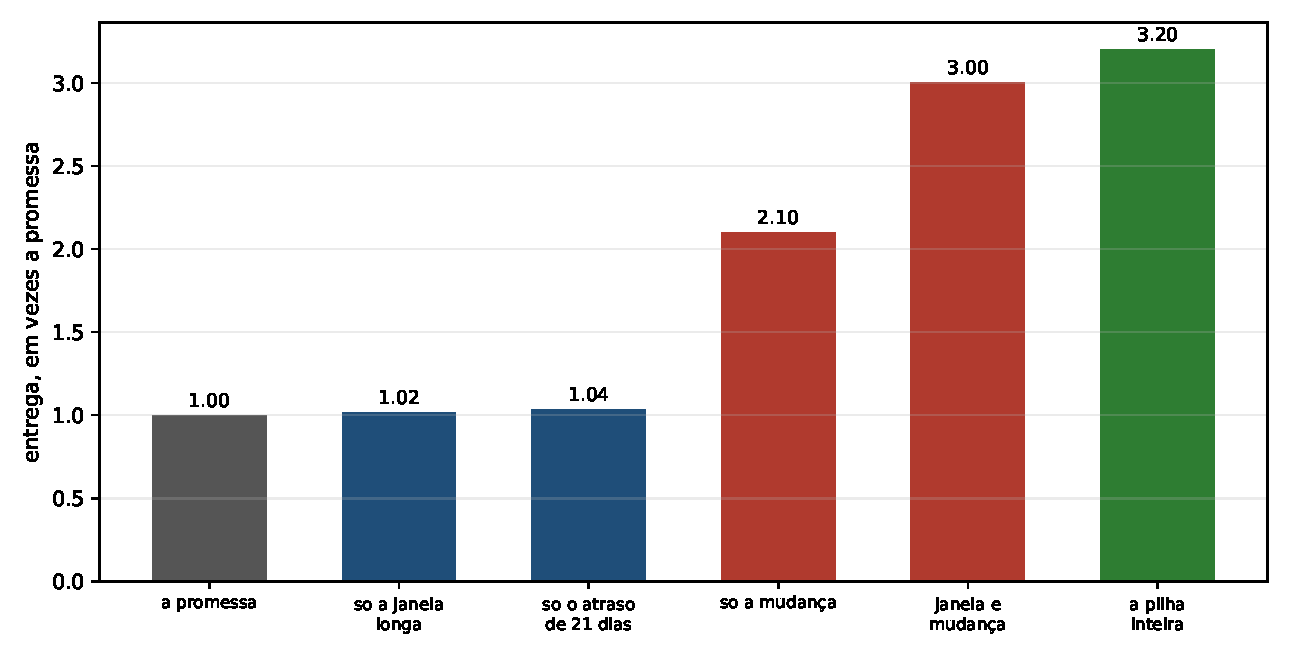
\includegraphics[width=\linewidth]{figuras/E20_o_fecho_2.pdf}
  \caption{A entrega de cada buraco sozinho e a da pilha inteira, em vezes a promessa. A barra verde é a
    mais alta das seis, e o que essa altura diz é o que o livro inteiro perseguiu: os buracos não se
    somam, eles se encaixam.}
  \label{fig:pilha}
\end{figure}

\section{O balanço}

O livro mediu preços em moedas diferentes, e vale olhar para eles na mesma página, cada um na sua.

\begin{table}[htbp]
  \centering
  \small
  \begin{tabular}{lll}
    \hline
    o que foi medido & o número & a moeda \\
    \hline
    a promessa do corte & \numPromessaPct{}\% dos dias & a fração \\
    o orçamento do alarme, no limiar \numVigiaLimiar{} & \numTrocaTrezeAnos{} anos por alarme falso & o tempo de mundo \\
    o que ele paga no tombo & \numTrocaTrezePagoPct{}\% do prejuízo & o prejuízo \\
    a memória que aprende & \numEsquecimentoMelhorMemoria{} dias, erro \numEsquecimentoMelhor{} & o erro \\
    o mundo que faltou & \numRecordeProbabilidade{} de um dia pior no ano & a probabilidade \\
    o atraso de um ano & \numAgoraRazaoDuzentosECinquentaEDois{} vezes a conta do corte & a fração \\
    a direção do tempo & \numDirecaoIndiceRazao{} desvios & o desvio \\
    quem cai primeiro & \numConjuntaDesvios{} desvios & o desvio \\
    a pilha dos buracos & \numFechoPilha{} vezes a promessa & a promessa \\
    \hline
  \end{tabular}
  \caption{Os preços que o livro mediu, cada um na moeda em que foi medido.}
  \label{tab:balanco}
\end{table}

A tabela diz o que o livro tem e o que ele não tem. Tem preço para quase tudo, e cada um na moeda
em que foi medido: a fração, o tempo de mundo, o prejuízo, o erro, a probabilidade, o desvio e a
promessa. E não tem câmbio entre as três moedas do fio condutor --- dados, trabalho e memória. As
conversões que apareceram são locais: a lei $k/(n+1)$ converte memória em cobertura dentro do corte;
a taxa de atualização converte trabalho em perda dentro do modelo da partilha; o horizonte de
recuperação converte memória em passado recuperável dentro do processo que declara o seu decaimento.
Cada uma vale no seu mundo, e nenhuma atravessa os outros.

A hipótese do fio condutor fica, então, com o veredito que a medição sustenta: \textbf{promessa e entrega
são a mesma pergunta em três lugares, e os três lugares não têm a mesma régua}. Quem tentar somar
dias de memória com dias de trabalho soma grandezas que não têm câmbio; quem mantiver as três
contas separadas e declaradas vai saber sempre o que prometeu e o que paga.

\section{O que fica}

Fica a resposta da pergunta da raiz, e ela cabe em três linhas.

\textbf{O que se pode garantir.} Uma promessa declarada, com o preço declarado ao lado: o instrumento
entrega \numFechoParadoLongaSemAtraso{} vezes a promessa de \numPromessaPct{}\% dos dias num mundo parado, o preço em alarmes falsos está na
\cref{tab:balanco}, e o que se paga quando o mundo muda está na \cref{tab:pilha}. Garantia sem preço
não é garantia, é frase.

\textbf{O que se pode medir.} A entrega, contra a promessa, sempre com a dispersão --- entre mundos
sorteados, entre pedaços da série, entre atrasos do dado. Uma medida sem o seu controle, sem a sua
dispersão ou sem a sua borda declarada é aritmética com nome de descoberta.

\textbf{O que se pode otimizar.} As bordas, e só elas: quanto passado entra na conta, de quando é o dado,
e onde a série começa e termina. Otimizar as bordas é barato e mede-se; otimizar o mundo é o que não
se compra, e os três capítulos do andar mostraram o preço de tentar.

Fica também o que o livro não fez. Não unificou as três contas. Não encontrou a lei que gera a
mudança, e mediu o que se pode fazer sem ela. E não prometeu nada sobre o mercado que não tenha
medido nos dados deste repositório. O que ele deixou é um conjunto de instrumentos com
preço: um corte declarado, um orçamento de alarmes, uma partilha de relógio, um esquecimento com
taxa, um desenho de intervenção com custo em dias, e a disciplina de declarar as bordas antes de
responder. Quem retomar o trabalho tem tudo isso; e tem, no primeiro capítulo, a mesma pergunta que
abriu o livro, agora com o preço ao lado.
